\section{ผลงานที่เกี่ยวข้อง}

จากงานนำเสนอ \cite[HAPS Strategy of Space Compass]{spacecompass}
กล่าวถึงความร่วมมือของบริษัท Airbus, NTT, DOCOMO,JSAT ในการส่งเสริมงานวิจัยและการพาณิชย์ในธุรกิจ Space RAN(Radio Access Network)
โดยเริ่มต้นจากการติดตั้งระบบ HAPS ในเครื่องบิน ชื่อว่า Zephyr ของบริษัท Airbus บินในชั้นบรรยากาศสตราโตสเฟียร์(Stratospher) 
และเริ่มการทดลองจริงโดยส่งคลื่นวิทยุไปสถานีเครือข่ายภาคพื้นดินโดยความถี่
UHF - 2GHz, 450MHz เพื่อวัดความสามารถในการกระจายสัญญาณ การทดลองนี้ใช้ระยะเวลา 18 วัน 
จึงสรุปผลการทดลองได้ว่าที่สัญญาณความถี่ 450MHz นั้นมีระยะการเชื่อมต่อสูงสุดอยู่ที่ 140 กม. 
\\
\begin{figure}[h]
\centering
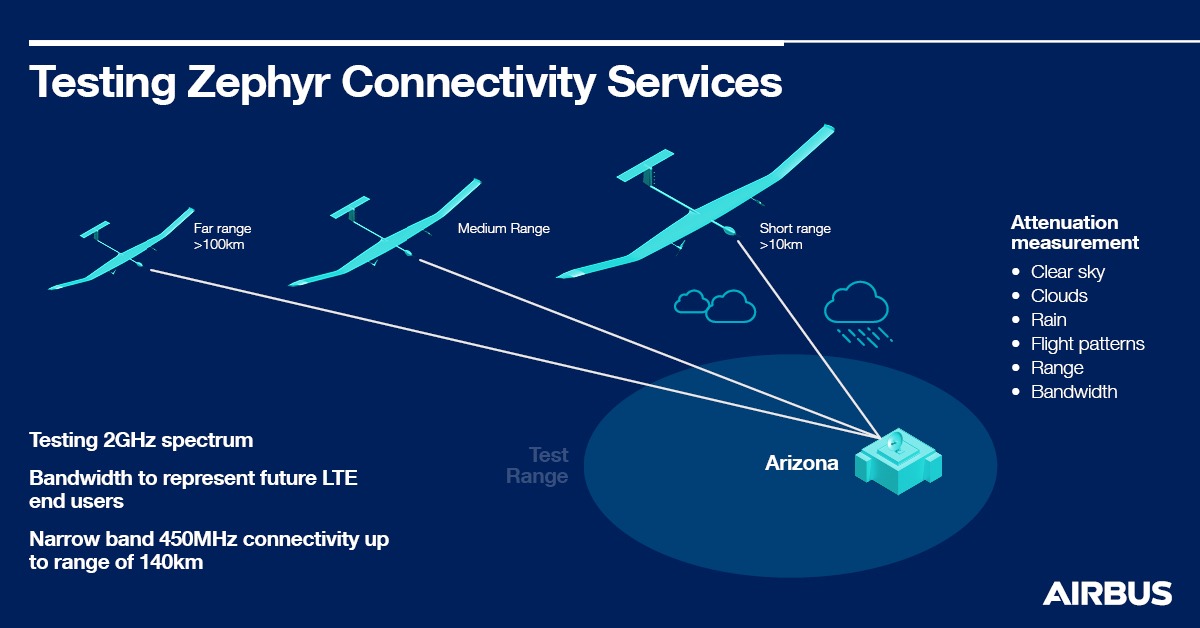
\includegraphics[width=0.5\textwidth]{Zephyr_Airbus.jpeg}
\end{figure}

จากงานวิจัย \cite[High Altitude Platform Systems: Towers in the Skies]{towers}
นำเสนอถึงความหลากหลายของ HAPS ที่ปรับเปลี่ยนได้ตามความต้องการในด้านพื้นที่ที่สัญญาณครอบคลุม ด้วยเทคโนโลยีเสาอากาศแบบใหม่ช่วยให้กำหนดทิศทางไปยังพื้นที่เป้าหมายที่ต้องการ กลายเป็นเครือข่าย
ประเภทหนึ่งชื่อว่า Fixed wireless access (FWA) เป็นเครือข่ายสัญญาณไร้สายประเภทหนึ่งที่ให้บริการอินเทอร์เน็ตความเร็วสูงแก่ประชาชนภาคครัวเรือน ในทางทฤษฎีแล้ว
FWA ผ่าน HAPS สามารถปลดล็อคขีดจำกัดการถ่ายโอนข้อมูลสูงสุด(Capacity)และความล่าช้า(Latency)ที่ต่ำกว่าเครือข่ายจากดาวเทียม
ทำให้อาจเป็นอีกหนึ่งทางเลือกนอกจากเครือข่ายสัญญาณแบบไฟเบอร์(Fibre-based)
\\
\begin{figure}[h]
\centering
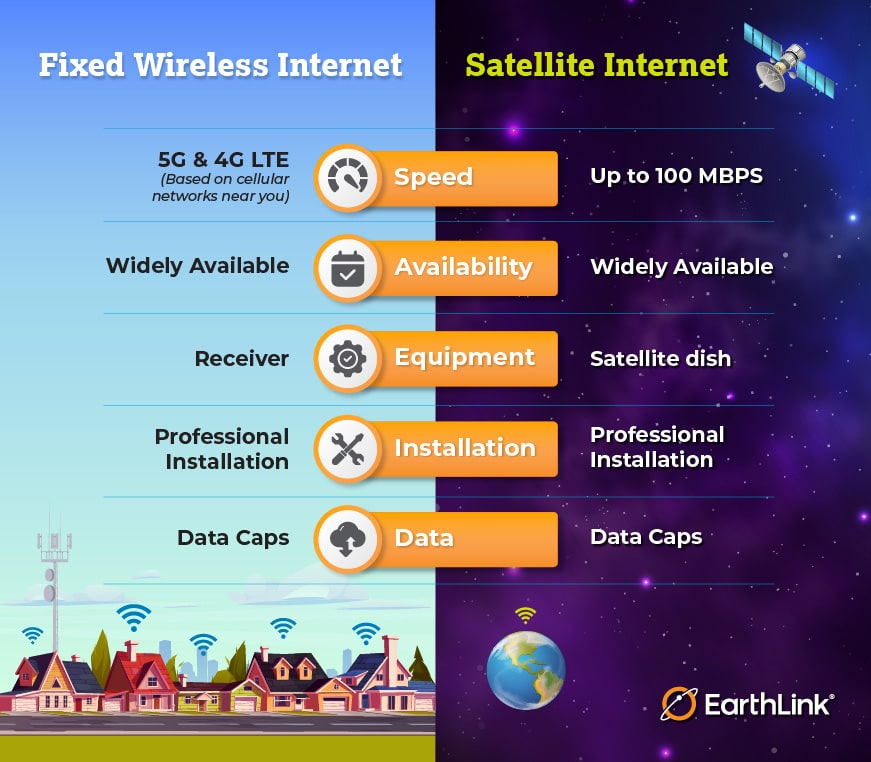
\includegraphics[width=0.5\textwidth]{wireless-vs-satellite-internet.jpg}
\end{figure}